\documentclass[slidestop,uncompress,mathserif,final]{beamer}

\usepackage{color, graphicx}
\usepackage[draft]{fixme}
\usepackage[utf8]{inputenc}
\usepackage{pgf}
%\usepackage{beamerthemesplit}

\usetheme{Singapore} 

% Util commands %
\newcommand{\pgl}[0]{Peter Gorm Larsen} 
\newcommand{\mail}[1]{{\small \texttt{#1}}}
\newcommand{\yellow}[1]{{\color{yellow} #1}}
\newcommand{\blue}[1]{{\color{blue} #1}}
\newcommand{\red}[1]{{\color{red} #1}}
\newcommand{\green}[1]{{\color{green} #1}}
\newcommand{\fixin}[1]{\fixme[inline]{\texttt{#1}}} 
\newcommand{\fixfo}[1]{\fixme[footnote]{\texttt{#1}}} 
\newcommand{\fixma}[1]{\fixme[margin]{\texttt{#1}}} 
\newcommand{\from}[1]{%
\noindent%
\begin{flushright}%
    \emph{\footnotesize #1}%
\end{flushright}%
} 

\title{An Overview of Overture and how tools for VDM are bootstrapped}

\subtitle{Rodin User and Developer Workshop}

\author[K. Lausdahl, M. Ferreira]{
  Kenneth Lausdahl \\
  \mail{kenneth AT lausdahl.com} \\
  Miguel Ferreira \\
  \mail{m.ferreira AT sig.nl}
}

\institute[IHA, SIG]{
  Aarhus School of Engineering\\
  Software Improvement Group
}

\pgfputat{\pgfxy(0,-6.5)}{\pgfbox[left,base]{
\includegraphics[width=2cm]{images/OMLlogoattempt.jpg}}}

\date{Southampton --- July 16 2009}

\begin{document}

\begin{frame}[c]
	\titlepage
\end{frame}

\begin{frame}[c]
  \frametitle{Outline}
  \tableofcontents %[pausesections] %[current,currentsubsection]
%  \tableofcontents[current]
\end{frame}

\section{The Overture Project}
\frame
{
  \frametitle{Introduction}

%\begin{block}<+->{Abstract}
%A short introduction to the Overture project showing how to bootstrap the tools for VDM. Short demo of the Editor and Debug execution.
%\end{block}
\begin{center}
  \begin{itemize}
	\itemsep=1cm
  		\item<1-> Vienna Development Method 
		\item<2-> Multi dialect (VDM-SL, VDM++ and VDM-RT).
  		\item<3-> VDM Tools
  \end{itemize}
\end{center}
}


\frame
{
  \frametitle{The Overture project}

\begin{block}<+->{Mission}
	Overture's mission is twofold: 
  \begin{itemize}
  		\item to provide an industrial-strength tool that supports the use of precise abstract models in software development, and 
  		\item to foster an environment that allows researchers and other interested parties to experiment with modifications and extensions to the tool.      

  \end{itemize}
\end{block}

The Overture tools are being developed by volunteers, researchers and students.
}


\subsection{Overview of the Overture Tools}
\frame
{
  \frametitle{Overview of the Overture Tools}

\begin{figure}[t]
\centering
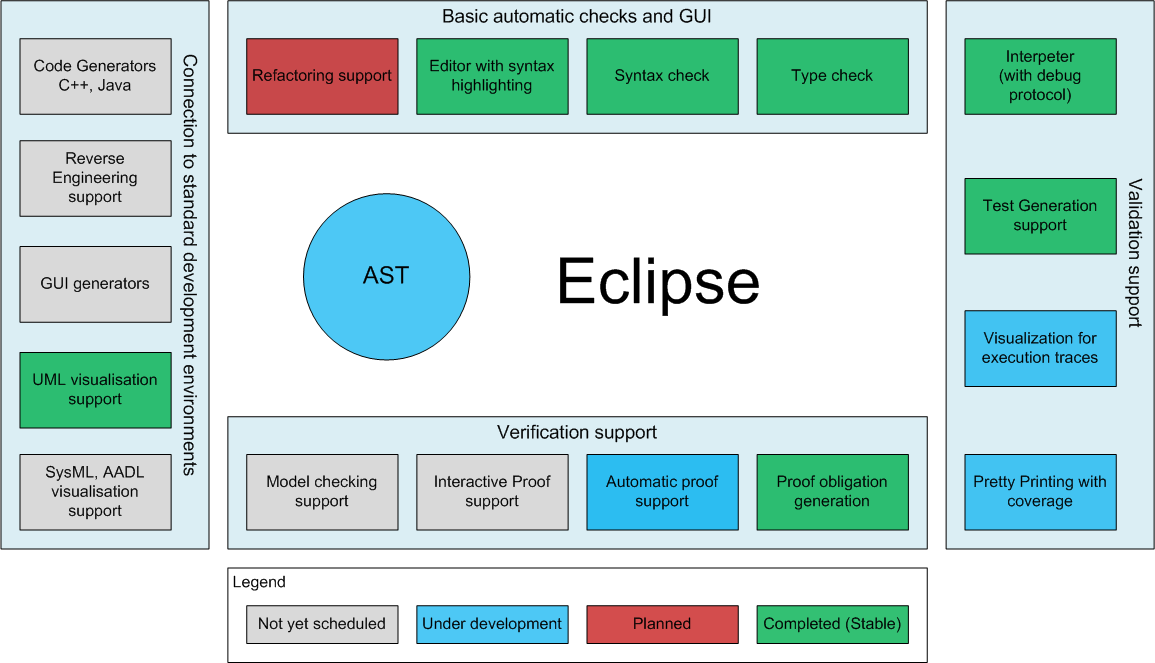
\includegraphics[width=\textwidth]{images/OvertureOverview}
%\caption{}
\label{fig:}
\end{figure}

}

\begin{frame}
	\frametitle{Overture components}
	\begin{columns}
		\column{.5\textwidth}
			\begin{block}{Basic automatic checks and GUI}
				{\scriptsize\begin{itemize}
				  \item Refactoring support.
				  \item Editor with syntax highlighting.
				  \item Syntax check.      
				  \item Type check.
				\end{itemize}}
			\end{block}
		\column{.5\textwidth}
			\begin{block}{Connections to standard development environments}
				{\scriptsize\begin{itemize}
			  \item Code Generators C++, Java.
			  \item Reverse Engineering support.
			  \item GUI generators.      
			  \item UML visualization support.
			  \item SysML, AADL visualization support.
				\end{itemize}}
			\end{block}
	\end{columns}
\end{frame}

\note{
	\begin{block}{Basic automatic checks and GUI}
		{\tiny\begin{itemize}
		  \item Refactoring support: Enabling easy refactoring e.g. rename a instance variable in a complete class.
		  \item Editor with syntax highlighting: Editor like Eclipse. Highlight all language specific keywords.
		  \item Syntax check: VDMJ Parser.
		  \item Type check: VDMJ Type checker.
		\end{itemize}}
	\end{block}
%		\column{.5\textwidth}
	\begin{block}{Connections to standard development environments}
		{\tiny\begin{itemize}
	  \item Code Generators C++, Java: Like VDM Tools code generator.
	  \item Reverse Engineering support: Going from e.g. Java to VDM. Prototype exists in VDM Tools
	  \item GUI generators: Automatic generation of basic GUI for the functions/operations in a VDM++ model.
	  \item UML visualization support: Bidirectional transformation VDM++ $\leftrightarrows$ Class / Sequence Diagrams.
	  \item SysML, AADL visualization support: Modeling languages.
			\begin{description}
				\item[SysML] Analysis, Verification, Validation.
				\item[AADL]  Analysis of Performance-critical properties.
			\end{description}
		\end{itemize}}
	\end{block}

}

\begin{frame}
	\frametitle{Components}

	\begin{columns}
	  \begin{column}{.5\textwidth}
	%	\column{.5\textwidth}
			\begin{block}{Validation support}
				{\footnotesize\begin{itemize}
				  \item Interpreter (with debug protocol).
				  \item Test generation support.
				  \item Visualization for execution traces.      
				  \item Pretty Printing with coverage.
				\end{itemize}}
			\end{block}
		  \end{column}
	  \begin{column}{.5\textwidth}
			\begin{block}{Verification support}
				{\footnotesize\begin{itemize}
					\item Proof obligation generation.
					\item Model checking support.
					\item Interactive Proof support.
					\item Automatic proof support.      
				\end{itemize}}
			\end{block}
		  \end{column}
		\end{columns}

\onslide<2->
  \begin{exampleblock}{Connection to Rodin}
The automatic proof support is current done in HOL but the GUI presentation of that will be difficult inside Eclipse. So an alternative connection to Rodin would be interesting if possible.
  \end{exampleblock}

\end{frame}




%\frame
%{
%  \frametitle{Overview of the Overture components}
%Main component categories:
%  \begin{itemize}
%  \item<1-> Basic automatic checks and GUI.
%  \item<2-> Connections to standard development environments.
%  \item<3-> Validation support.      
%  \item<4-> Verification support.
%  \end{itemize}
%}
%
%\frame
%{
%  \frametitle{Basic automatic checks and GUI}
%
%  \begin{itemize}
%  \item<1-> Refactoring support.
%  \item<1-> Editor with syntax highlighting.
%  \item<1-> Syntax check.      
%  \item<1-> Type check.
%  \end{itemize}
%}
%
%\frame
%{
%  \frametitle{Connections to standard development environments}
%
%  \begin{itemize}
%  \item Code Generators C++, Java.
%  \item Reverse Engineering support.
%  \item GUI generators.      
%  \item UML visualization support.
%  \item SysML, AADL visualization support.
%  \end{itemize}
%}

%\frame
%{
%  \frametitle{Validation support}
%
%  \begin{itemize}
%  \item Interpreter (with debug protocol).
%  \item Test generation support.
%  \item Visualization for execution traces.      
%  \item Pretty Printing with coverage.
%  \end{itemize}
%}
%
%\frame
%{
%  \frametitle{Verification support}
%
%  \begin{itemize}
%  \item Model checking support.
%  \item Interactive Proof support.
%  \item Automatic proof support.      
%  \item Proof obligation generation.
%  \end{itemize}
%
%Somewhere on this slide the Rodin tool should be mentioned.
%}


\section{Tool Set}

\begin{frame}
  \frametitle{Outline}
  \tableofcontents[current]
\end{frame}

\subsection{Components}
\frame
{
  \frametitle{VDMJ}

  \begin{block}{Features}
	\begin{itemize}
		\item Syntax check.      
		\item Type check.
		\item Interpreter (with debug protocol).
		\item Pretty Printing with coverage (partly).
		\item Test generation support.
		\item Proof obligation generation.
		\item Multi dialect: VDM-SL, VDM++ and VDM-RT
  \end{itemize}
  \end{block}
}

\subsection{Eclipse integration}
\frame
{
  \frametitle{Editor}

  \begin{block}{Features}
	\begin{itemize}
	  \item Editor with syntax highlighting.
	  \item Syntax check.      
	  \item Type check.
	  \item UML visualization support.
	  \item Interpreter.
	  \item Test generation support.
  \end{itemize}
  \end{block}
}

\frame
{
  \frametitle{Editor Main view}

\begin{figure}[t]
\centering
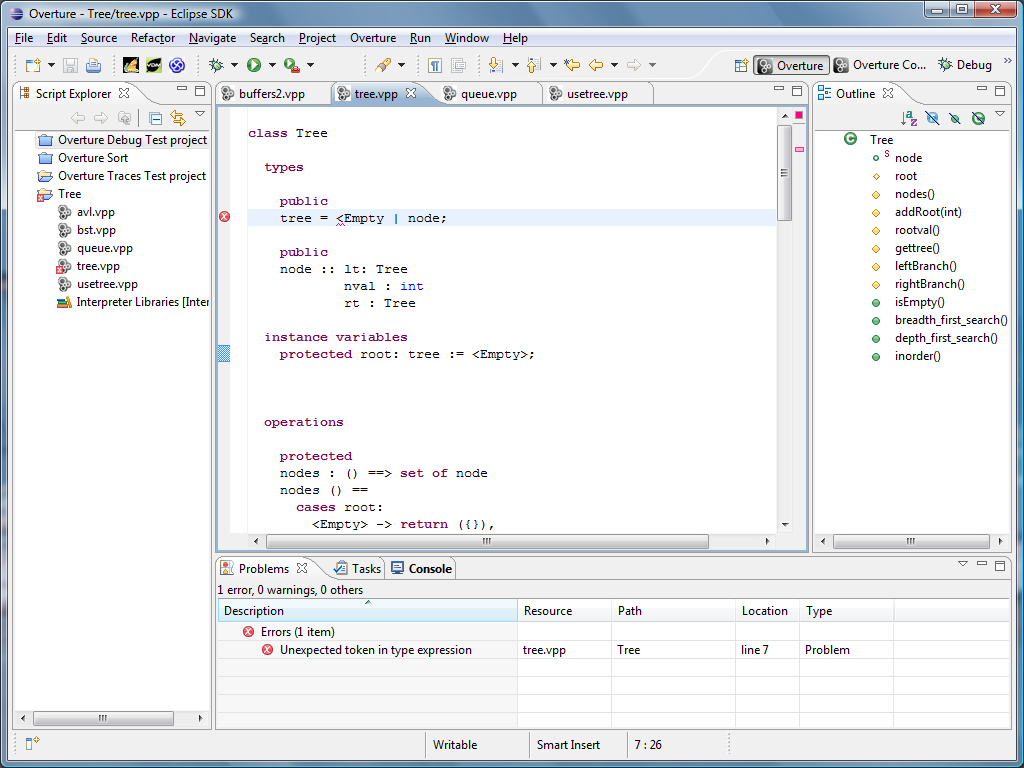
\includegraphics[width=0.8\textwidth]{images/EditorOverview}
%\caption{}
\label{fig:}
\end{figure}
}

\frame
{
  \frametitle{Demo}

  \begin{itemize}
  \item \href{http://mt.lausdahl.com/downloads/ScreenCasts/DemoOvertureDebugger/}{Overture Debugger.}     

  \end{itemize}
}


\section[Bootstrapping Tools for VDM]{Bootstrapping Tools for VDM --- Past and Present}
\label{sec:bootstrapping}

\begin{frame}[c]
  \frametitle{Outline}
  \tableofcontents[current]
\end{frame}

\subsection{Bootstrapping}
\begin{frame}[c]
  \frametitle{Bootstrapping}
  \framesubtitle{Compilers}


  \begin{quotation}
	``Bootstrapping is a term used in computer science to describe the techniques involved in \textbf{writing a compiler} (\dots) in the \textbf{target programming language} which \textbf{it is intended to compile}.''
  \end{quotation}
  \from{From Wikipedia, the free encyclopedia}
\end{frame}

\begin{frame}[t]
  \frametitle{Bootstrapping}
  \framesubtitle{How is it done?}

  \pause
  \begin{itemize}
	\item How to produce the first \alert{compiler} for a new \alert{language}?
  \end{itemize}

  \vspace{\fill}

  \pause
  \begin{block}{Niklaus Wirth --- the first Pascal compiler}
  \begin{itemize}
	\itemsep=.5cm
	\item Used a \alert{different language}  --- first implementation was written in Fortan;
	  \pause
	\item \alert{Manually compiled} the compiler --- second implementation was written in Pascal and hand compiled.
  \end{itemize}
  \end{block}
\end{frame}

\subsection[VDMTools]{History of VDMTools Bootstrapping --- \pgl~\cite{Larsen01}} 
\label{sec:vdmtools}



\begin{frame}[c]
  \frametitle{Architecture}

  \only<1> {
  \framesubtitle{Overview}
  \begin{center}
    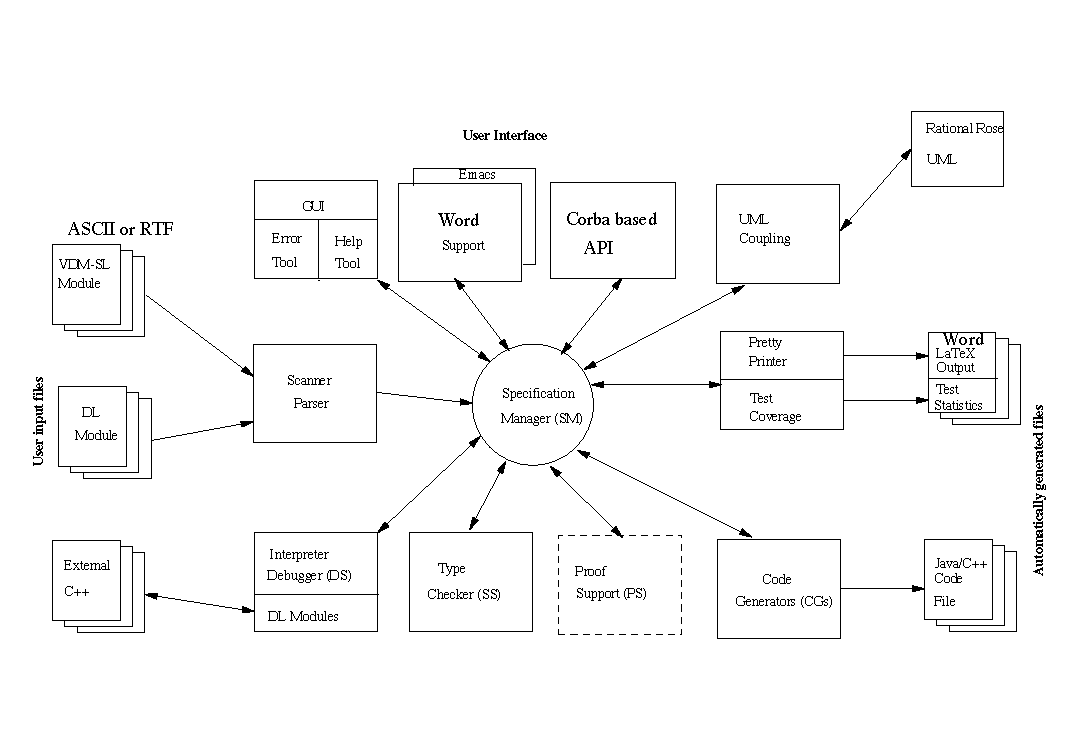
\includegraphics[width=\textwidth]{images/vdmtools_arch.pdf}
  \end{center}
  }
  \only<2> {
  \framesubtitle{Conventional development}
   \begin{center}
    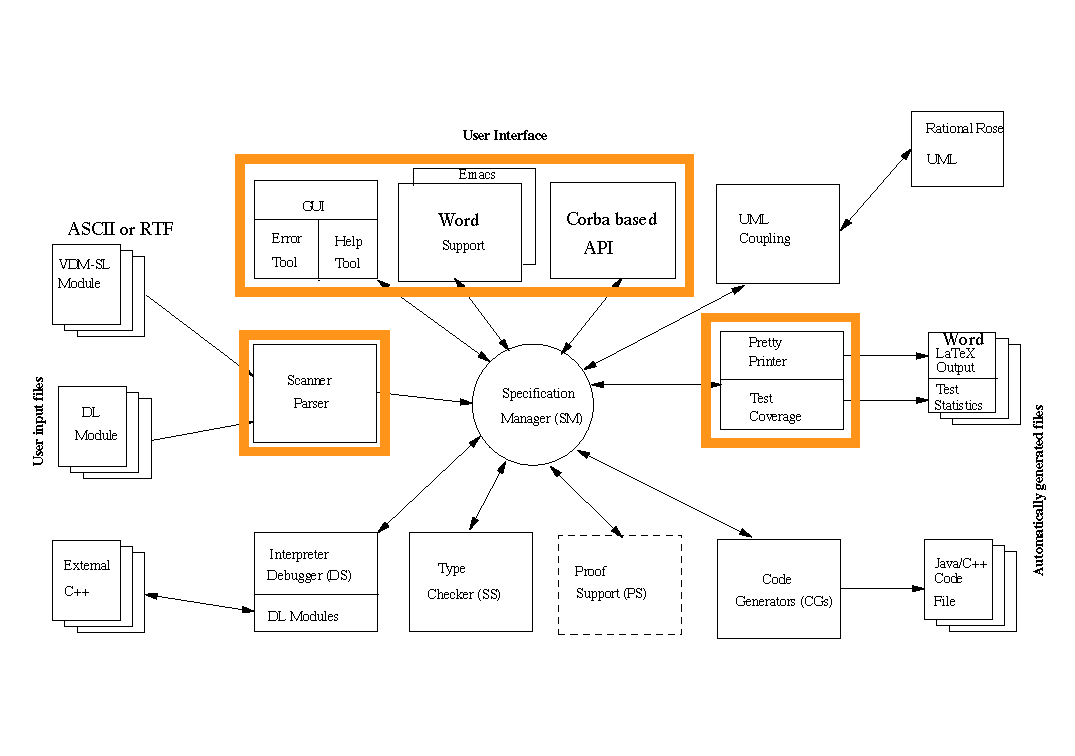
\includegraphics[width=\textwidth]{images/vdmtools_arch_conv_dev.pdf}
  \end{center}
  }
  \only<3>{
  \framesubtitle{Formally specified}
  \begin{center}
    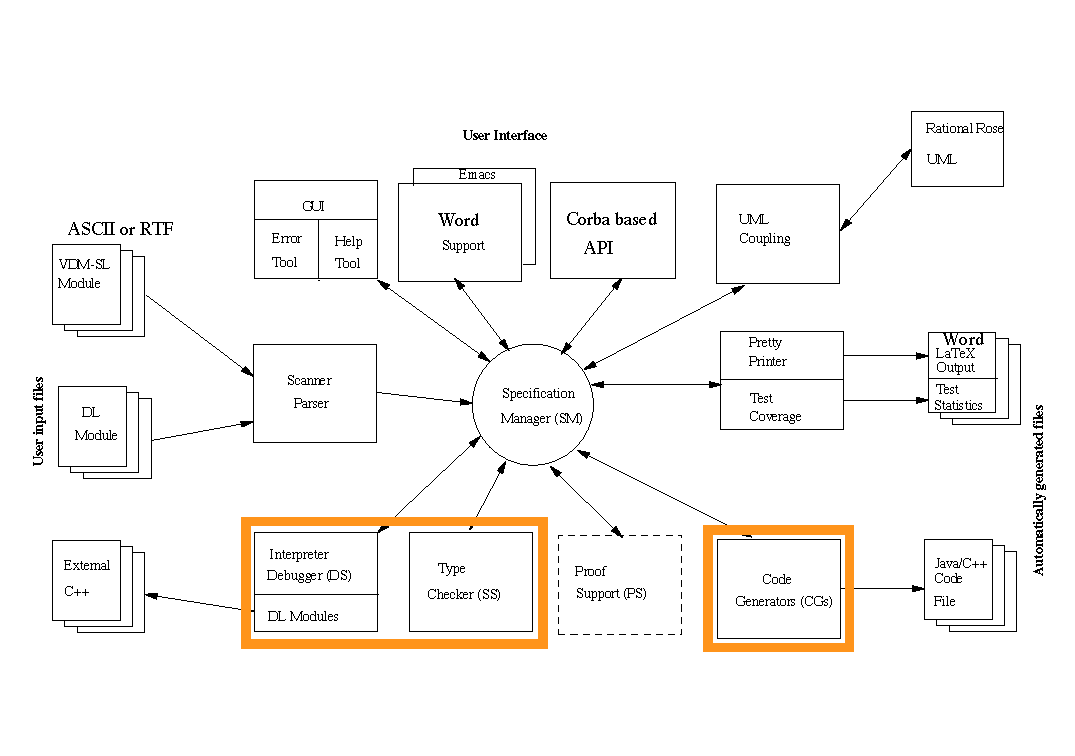
\includegraphics[width=\textwidth]{images/vdmtools_arch_spec.pdf}
  \end{center}
  }
  \only<4>{
  \framesubtitle{Generated code}
  \begin{center}
    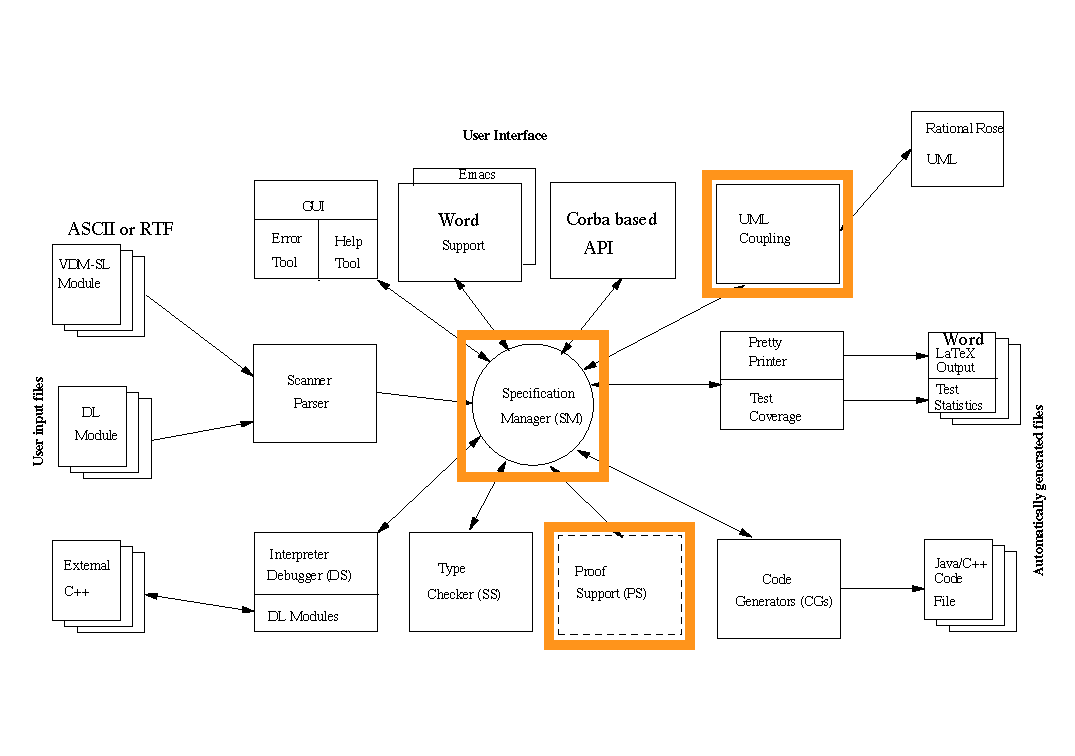
\includegraphics[width=\textwidth]{images/vdmtools_arch_cg.pdf}
  \end{center}
  }
\end{frame}


\begin{frame}[c]
  \frametitle{Bootstrapping}
  %\framesubtitle{Test and improvement --- \emph{\pgl~\cite{Larsen01}}}

  \only<1>{
  \framesubtitle{Test and improvement}
 
  \begin{center}
    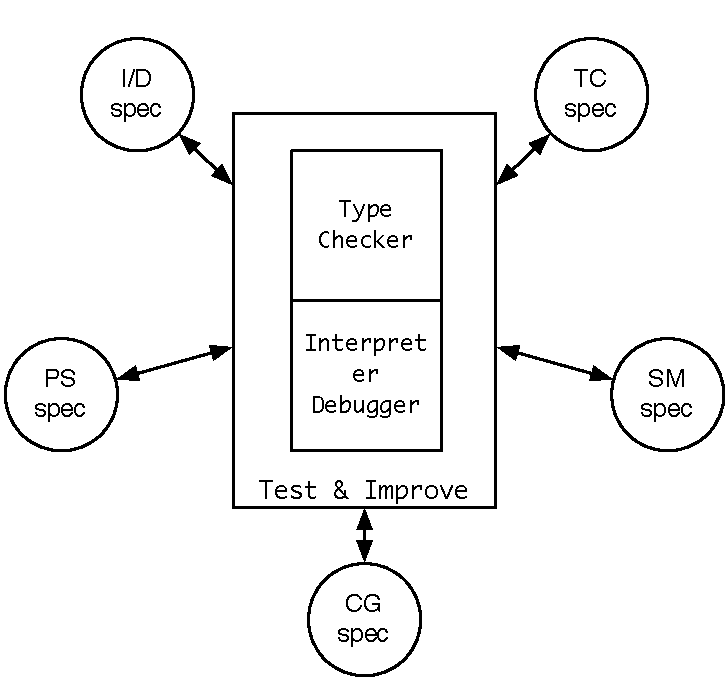
\includegraphics[width=.6\textwidth]{images/test_improve.pdf}
  \end{center}
  }
 \only<2>{
  \framesubtitle{Tool generation}
  \begin{center}
    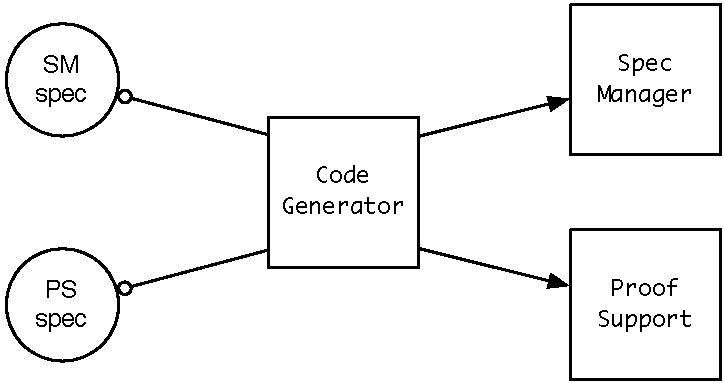
\includegraphics[width=.7\textwidth]{images/code_gen.pdf}
  \end{center}
  }
 \only<3>{
  \framesubtitle{Tool generation}
  \begin{center}
    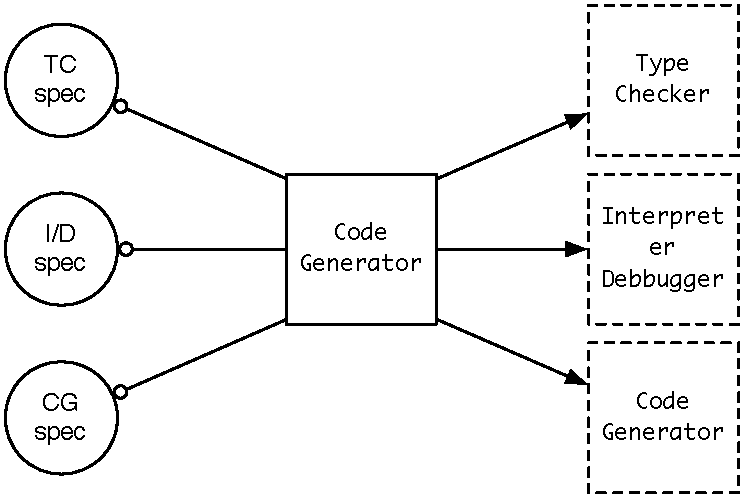
\includegraphics[width=.7\textwidth]{images/code_gen2.pdf}
  \end{center}
  }
\end{frame}


\subsection[Overture]{Bootstrapping Overture Tools}
\label{sec:overture}

\begin{frame}[c]
  \frametitle{Architecture}
  \framesubtitle{Overview}

  \begin{center}
    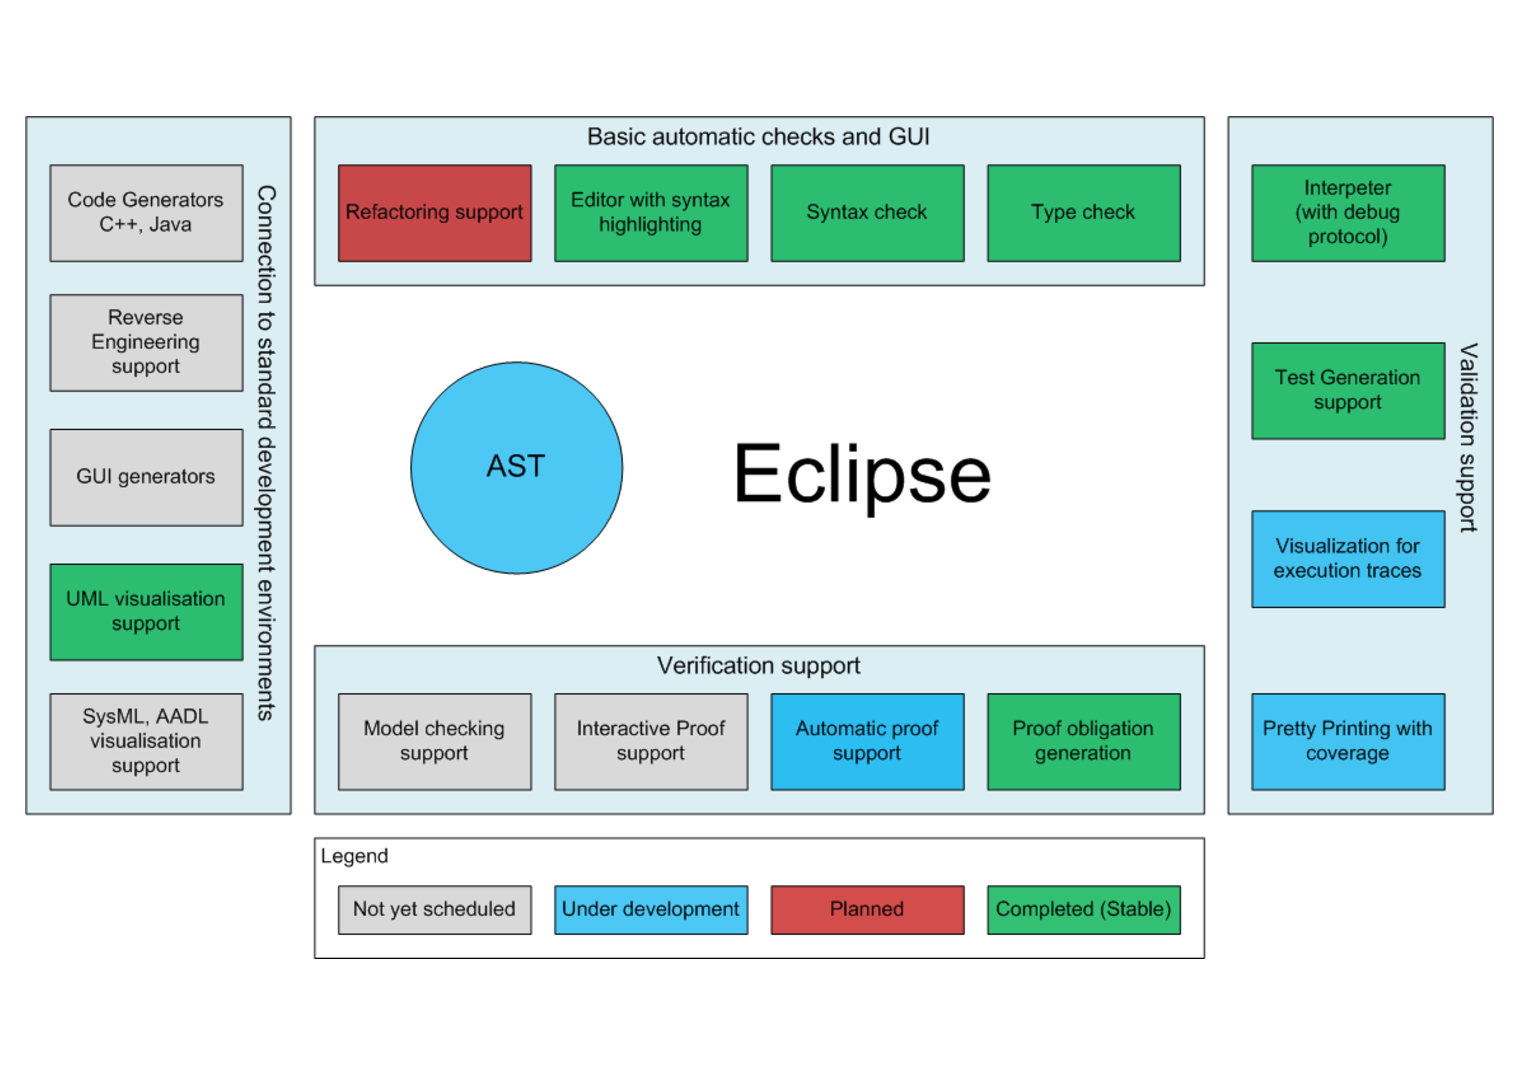
\includegraphics[width=\textwidth]{images/overture_arch.pdf}
  \end{center}
\end{frame}

\begin{frame}[c]
  \frametitle{Architecture}

  \only<1> {
  \framesubtitle{Conventional development}
  \begin{center}
    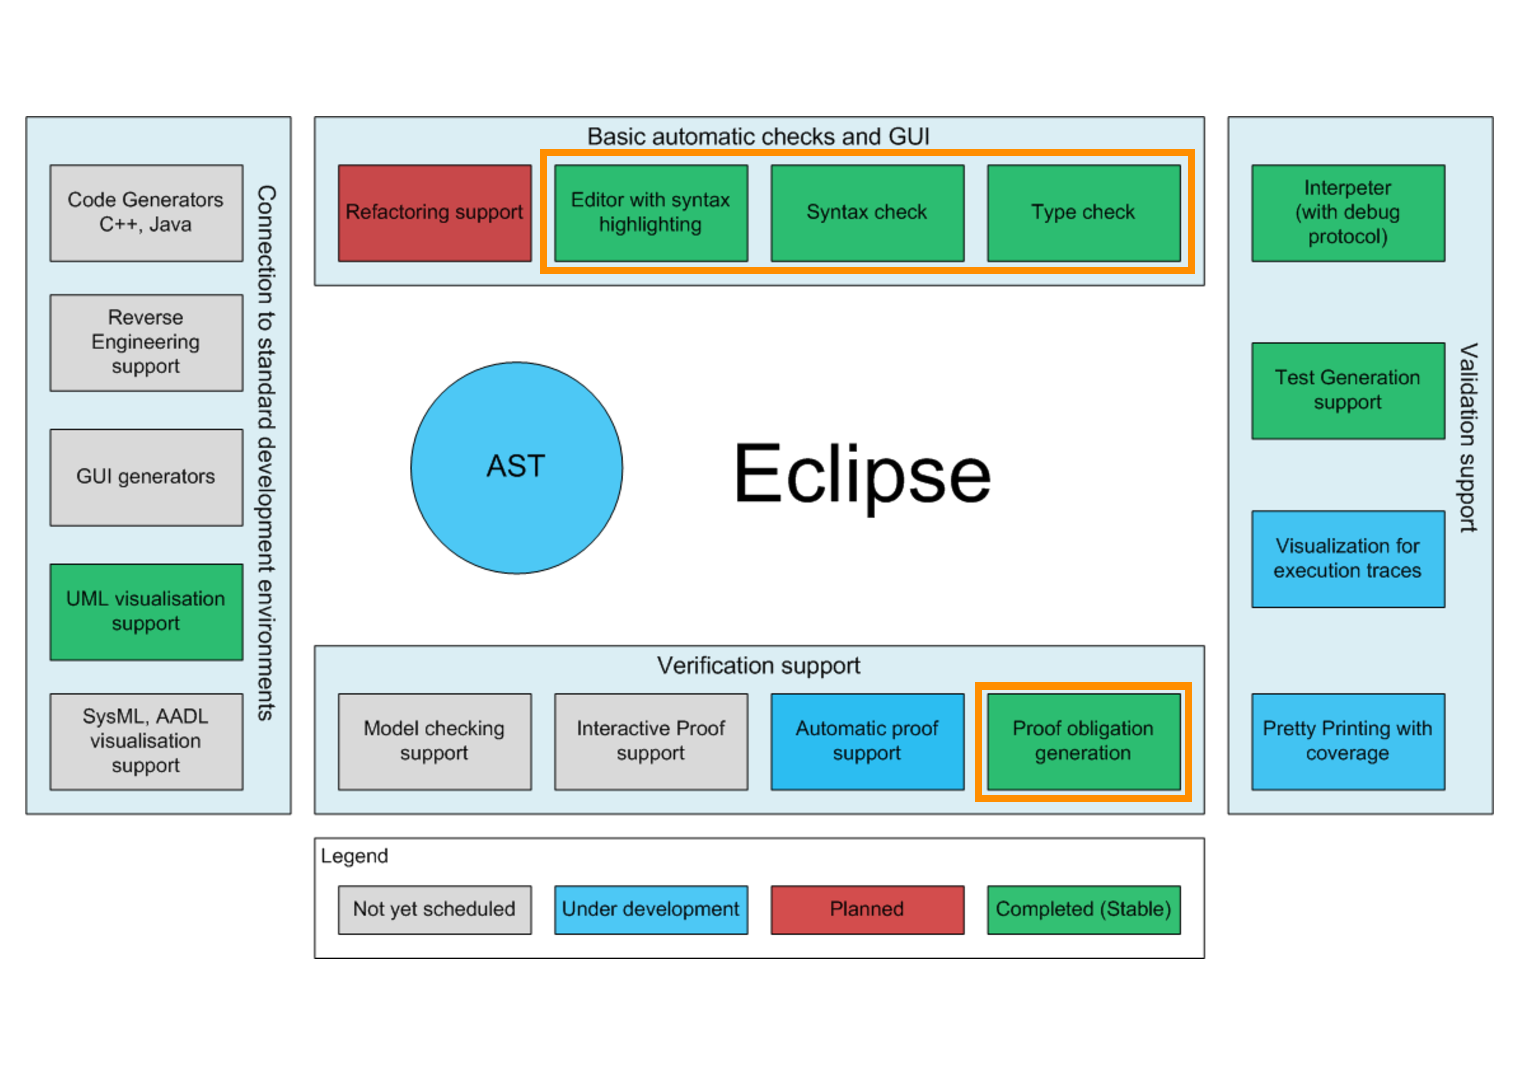
\includegraphics[width=\textwidth]{images/overture_arch_conv_dev.pdf}
  \end{center}
  }
  \only<2>{
  \framesubtitle{Formally specified}
  \begin{center}
    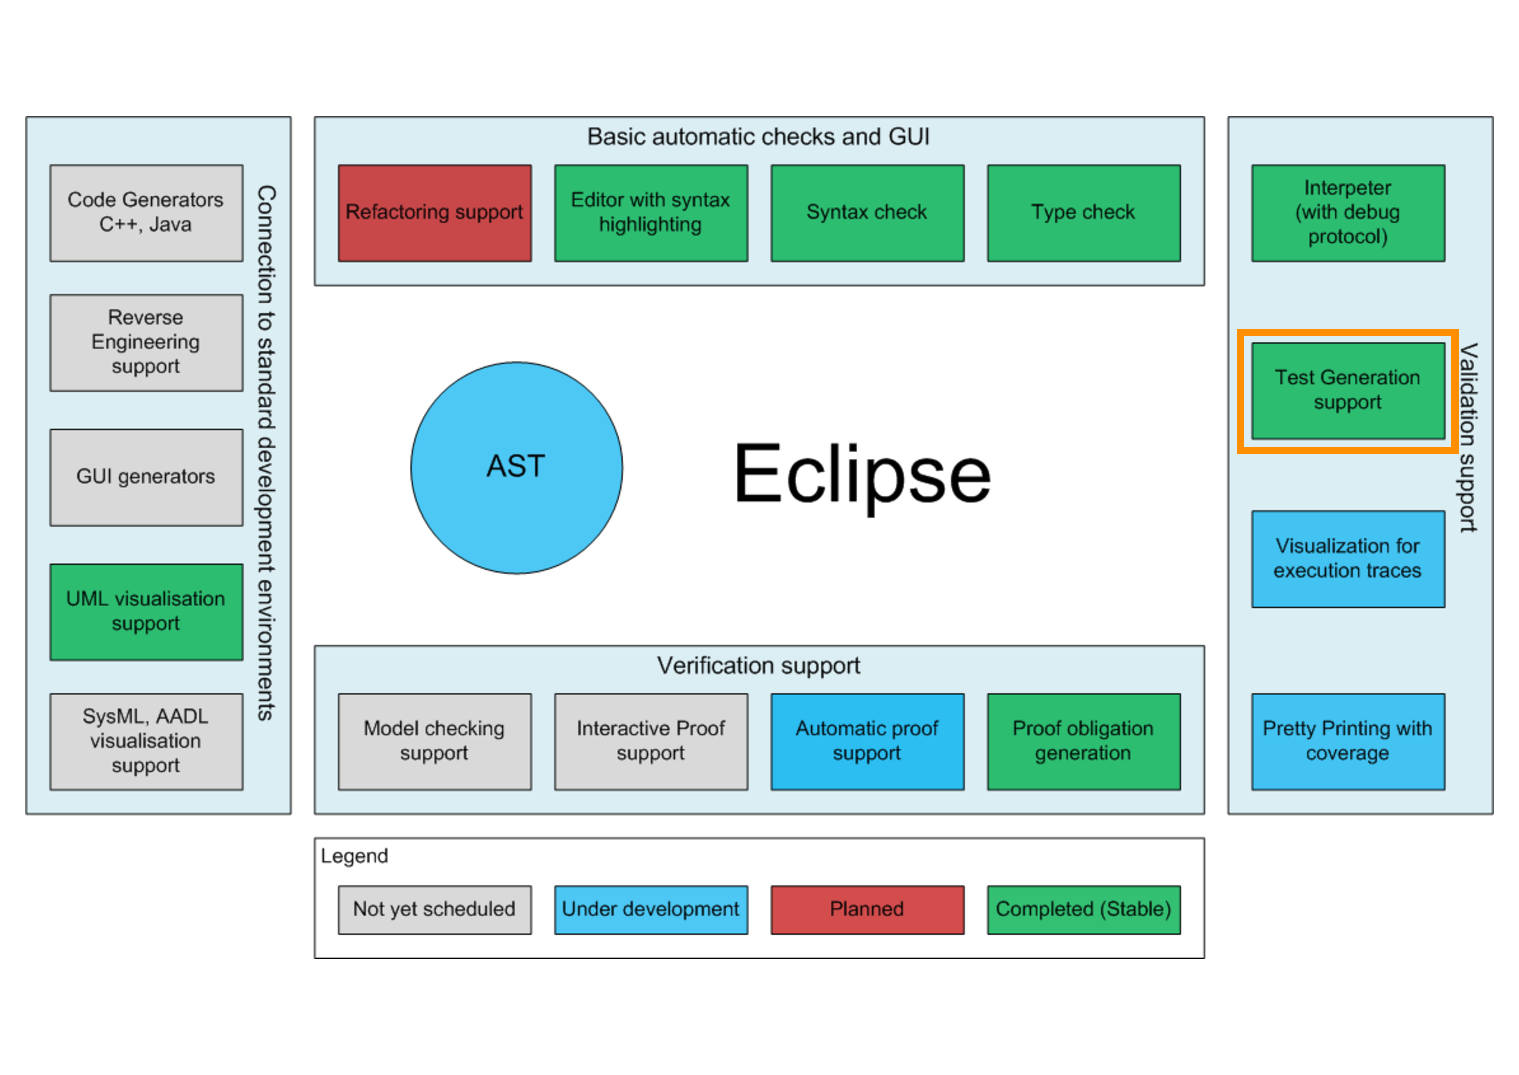
\includegraphics[width=\textwidth]{images/overture_arch_spec.pdf}
  \end{center}
  }
  \only<3>{
  \framesubtitle{Generated code}
  \begin{center}
    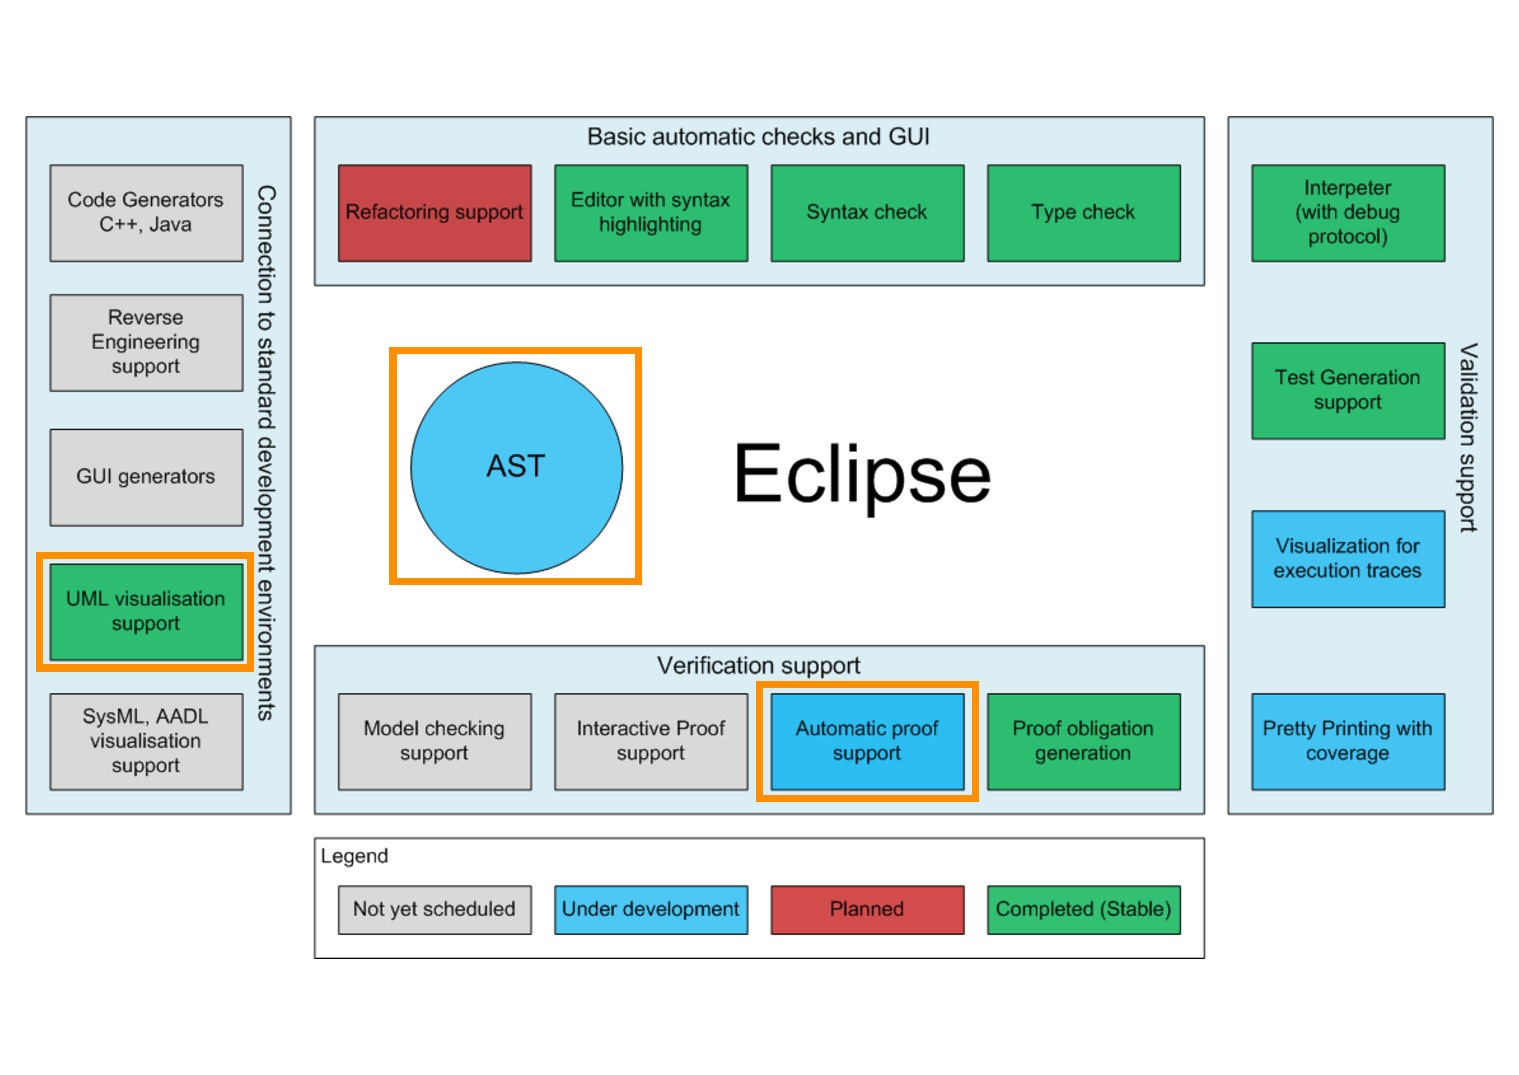
\includegraphics[width=\textwidth]{images/overture_arch_cg.pdf}
  \end{center}
  }
\end{frame}


\begin{frame}[c]
  \frametitle{Bootstrapping}

  \only<1>{
  \framesubtitle{AST Generation}
  \begin{center}
    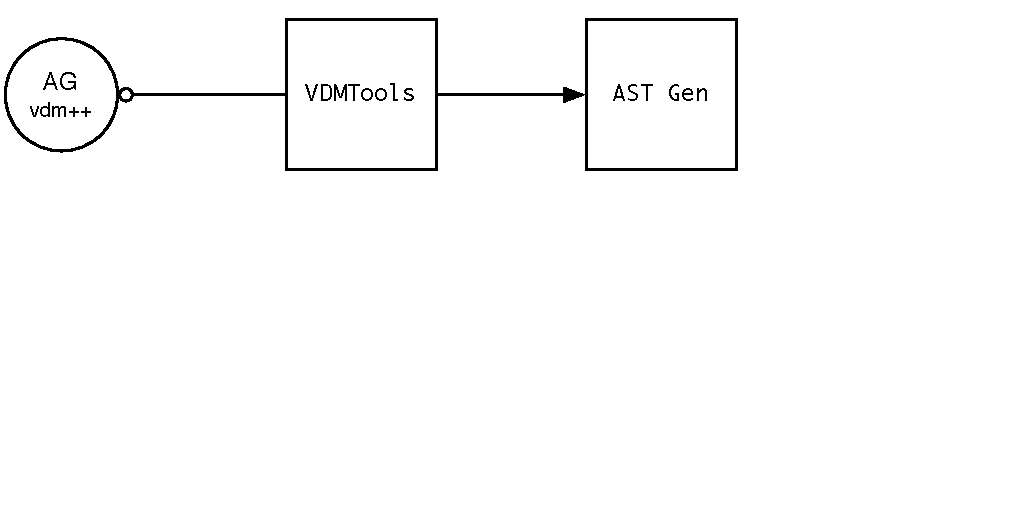
\includegraphics[width=\textwidth]{images/ast_gen_oml_ast_gen.pdf}
  \end{center}
  }
  \only<2>{
  \framesubtitle{AST Generation}
  \begin{center}
    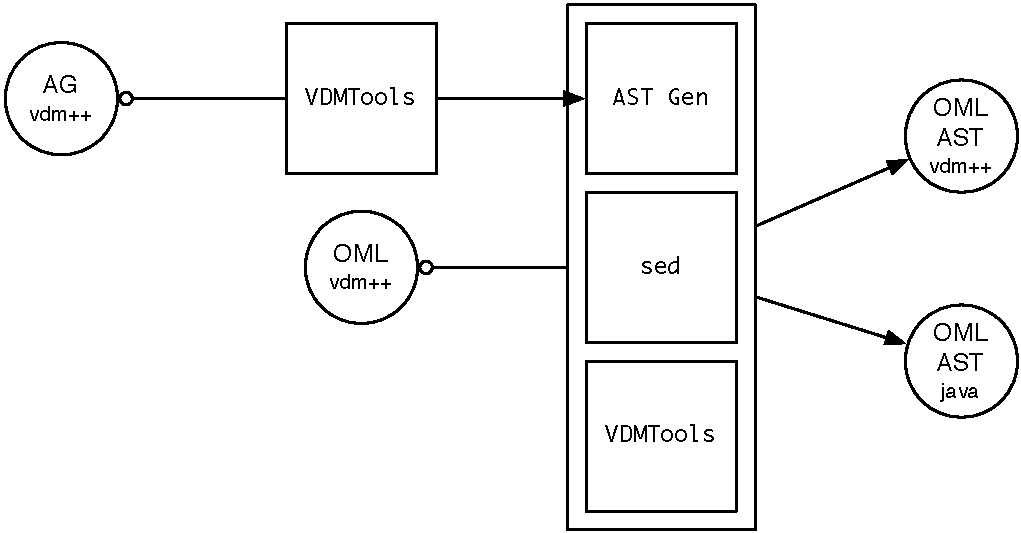
\includegraphics[width=\textwidth]{images/ast_gen_oml_ast_gen_2.pdf}
  \end{center}
  }
  \only<3>{
  \framesubtitle{Component Generation}
  \begin{center}
    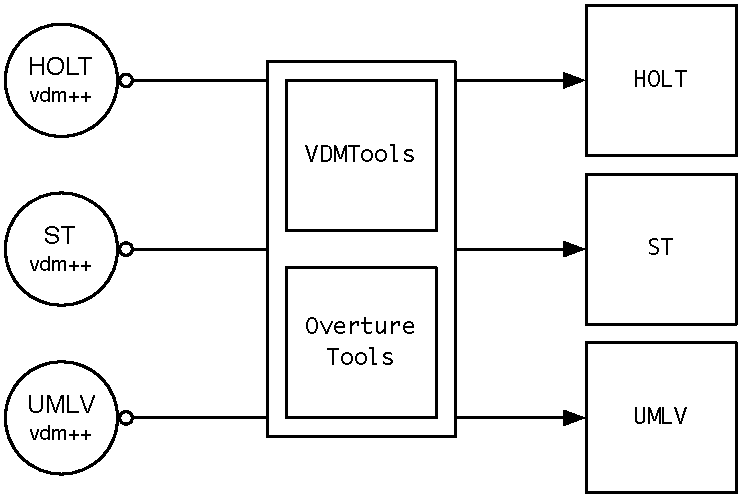
\includegraphics[width=.8\textwidth]{images/ovt_bootstrap.pdf}
  \end{center}
  }

\end{frame}


\begin{frame}[plain,c]
  \begin{center}
	\LARGE \structure{Thank you!}

	\vspace{2cm}
	\href{www.overturetool.org}{www.overturetool.org}
\end{center}
\end{frame}


\bibliographystyle{plain}
\bibliography{mf}



\end{document}